

\documentclass[11pt,english,ngerman, headsepline]{scrreprt}
\usepackage{lmodern}
\renewcommand{\sfdefault}{lmss}
\renewcommand{\ttdefault}{lmtt}
\usepackage[T1]{fontenc}

\usepackage{listings}

\usepackage[utf8]{inputenc} \usepackage[a4paper]{geometry}
\geometry{verbose,tmargin=3cm,bmargin=3cm,lmargin=3cm,rmargin=2.75cm,headheight=1cm,headsep=0.666cm,footskip=1cm}
\setcounter{secnumdepth}{3}
\setcounter{tocdepth}{3}
\setlength{\parskip}{\medskipamount}
\setlength{\parindent}{0pt}
\usepackage{babel}
  \usepackage{tipa}
\usepackage{verbatim} 
\usepackage{float}  
\usepackage{url}
\usepackage{graphicx}
\usepackage{setspace}
\usepackage[square,sort,numbers]{natbib} \usepackage[utf8]{inputenc}
\usepackage{graphicx} 
\usepackage[xindy,toc]{glossaries}
 
 
 
\setstretch{1.4}
\usepackage[usenames,dvipsnames]{color}
\usepackage[unicode=true, 
 bookmarks=true,bookmarksnumbered=false,bookmarksopen=true,bookmarksopenlevel=2,
 breaklinks=false,pdfborder={0 0 0},backref=false,colorlinks=false]
 {hyperref}
\hypersetup{pdftitle={MDT},
 pdfauthor={Nils M. Petersohn}}
 
\makeatletter

%%%%%%%%%%%%%%%%%%%%%%%%%%%%%% LyX specific LaTeX commands.
\providecommand{\LyX}{L\kern-.1667em\lower.25em\hbox{Y}\kern-.125emX\@}
%% Because html converters don't know tabularnewline
\providecommand{\tabularnewline}{\\}

%%%%%%%%%%%%%%%%%%%%%%%%%%%%%% Textclass specific LaTeX commands.
\newenvironment{lyxcode}
{\par\begin{list}{}{
\setlength{\rightmargin}{\leftmargin}
\setlength{\listparindent}{0pt}% needed for AMS classes
\raggedright
\setlength{\itemsep}{0pt}
\setlength{\parsep}{0pt}
\normalfont\ttfamily}%
 \item[]}
{\end{list}}




\usepackage{multirow}

 
%%%%%%%%%%%%%%%%%%%%%%%%%%%%%% User specified LaTeX commands.
%% Flexibles Seitenlayout
\usepackage[automark]{scrpage2}

%% Mehrspaltenlayout ermöglichen
\usepackage{multicol}

%% Unterst\"utzung f\"ur Farben
\usepackage{color}

%% Schönere Tabellen
\usepackage{booktabs, longtable}

%% Schönerer Blocksatz
\usepackage{microtype}
%% Mehr Platz zwischen Überschrift und Tabelle
\newcommand{\@ldtable}{}
\let\@ldtable\table
\renewcommand{\table}{ %
    \setlength{\@tempdima}{\abovecaptionskip} %
    \setlength{\abovecaptionskip}{\belowcaptionskip} %
    \setlength{\belowcaptionskip}{\@tempdima} %
    \@ldtable %
}

%% Verschiedene Symbole und Zeichen wie (c), ¤
\usepackage{textcomp}

%% Fehlerkorrektur f\"ur Marginalien
\usepackage{fixltx2e }%,mparhack

%% Deutsche Kurzfassung und englisches Abstract auf eine Seite
\renewenvironment{abstract}{
    \@beginparpenalty\@lowpenalty
        \begin{center}
            \normalfont\sectfont\nobreak\abstractname
        \end{center}
    \@endparpenalty\@M
}{
    \par
}

%% Alle Seiten vor dem Inhaltsverzeichnis sind römisch nummeriert
\pagenumbering{roman}
\let\myTOC\tableofcontents
\renewcommand\tableofcontents{
    \begin{spacing}{1.1}
    \myTOC
    \end{spacing}
    \clearpage
    \pagenumbering{arabic}
}

%% Kopfzeile um Logo erg\"anzen
\clearscrheadfoot
\ohead{\\\headmark}
\ihead{
\includegraphics[scale=0.25]{pics/FH-Logo-only-gray}}%\pagemark}
\ofoot[\pagemark]{\pagemark}

%% Randnotizen anpassen
\setlength{\marginparwidth}{22mm}
\let \oldmarginpar = \marginpar
\renewcommand{\marginpar}[1]{%
    \-\oldmarginpar[\raggedleft\footnotesize\sf #1]%
        {\raggedright\footnotesize\sf #1%
    }}

%% Zitate am Kapitelanfang
%\usepackage{epigraph}
%\setlength{\epigraphwidth}{9cm}

%% Code-Block-Formatierung
\lstdefinestyle{default}{ %
    backgroundcolor={\color[rgb]{0.95,0.95,0.95}}, %
    basicstyle={\small\ttfamily}, %
    breaklines=true, %
    frame=l, %
    language={[Sharp]C}, %
    lineskip=-0.1pt, %
    numbers=left, %
    rulecolor={\color[rgb]{0.5,0.5,0.5}}, %
    xleftmargin={0.75cm}, %
    xrightmargin={0cm} %
}
\lstdefinelanguage{JavaScript} {
	morekeywords={
		break,const,continue,delete,do,while,export,for,in,function,
		if,else,import,in,instanceOf,label,let,new,return,switch,this,
		throw,try,catch,typeof,var,void,with,yield
	},
	sensitive=false,
	morecomment=[l]{//},
	morecomment=[s]{/*}{*/},
	morestring=[b]",
	morestring=[d]'
}

\lstset{
	frame=tb,
	framesep=5pt,
	basicstyle=\footnotesize\ttfamily,
	showstringspaces=false,
	keywordstyle=\ttfamily\bfseries\color{CadetBlue},
	identifierstyle=\ttfamily,
	stringstyle=\ttfamily\color{OliveGreen},
	commentstyle=\color{GrayBlue},
	rulecolor=\color{Gray},
	xleftmargin=5pt,
	xrightmargin=5pt,
	aboveskip=\bigskipamount,
	belowskip=\bigskipamount
}
\makeatother

\setlength{\parindent}{5pt} 
\setlength{\parskip}{1ex}

\parindent 0pt

\begin{document} 


\titlepage

\begin{center}

\includegraphics[width=5cm]{pics/FH-Logo}\vspace{0.5cm}

\par\end{center}

\noindent \begin{center}
\textsf{\textbf{\Large Fachbereich Informatik und Medien - \\
Wissenschaftliches Arbeiten und Schreiben - Master Inf. Prof. Loose
WS 2011/12}}\\ \textsf{\large }\\
\vspace{1cm}

\par\end{center}

\begin{center}
\textsf{\textbf{\huge Untersuchung des sprachorientierten
Programmierparadigmas anhand von Metaprogrammierung und einer damit
erstellten DSL für Preispoitik in einem Boardinghaus.\\
}}\textsf{}\\ \textsf{}\\ 

\par\end{center}{\Large \par}

\vspace{2cm}


\noindent \begin{center}
{\huge }\begin{tabular}{rl}
Vorgelegt von: & Nils Petersohn B.Sc. \tabularnewline am: &
29.02.2012.\tabularnewline
\end{tabular}
\par\end{center}{\huge \par}

\vspace{1cm}

\begin{abstract}
 
Sprachorientierte Programmierung ist in dieser Arbeit betrachtet wurden.
Dazu wurde eine DSL mit Hilfe der Groovy-MOP erstellt, um daran das Paradigma
zusammen mit dem Domänenexperten unter folgenden Gesichtspunkten zu bewerten:
Lesbarkeit, intuitivem Verständnis und Flexibilität. 
Der Autor beschreibt intensiv die Erstellung der DSL und die
Metaprogrammierungs-Leistungsträger der gewählten Programmiersprache.

\end{abstract}
 

\noindent \begin{center}
\medskip{}
\begin{tabular}{rl}
\tabularnewline
\end{tabular}
\par\end{center}

\newpage{}

%
\begin{comment}
leere Seite nach dem Titelblatt

dann Aufgabenstellung
\end{comment}


\begin{comment}
%\pagestyle{scrheadings}    %Kopfzeile ein

\noindent \begin{center}
\textsf{\textbf{\large Selbstst\"andigkeitserkl\"arung}}
\par\end{center}{\large \par}

\noindent Hiermit erkl\"are ich, dass ich die vorliegende Arbeit zum
Thema

\smallskip{}


\noindent \begin{center}
\textsf{Medienverwaltung mit Eclipse und Equinox}
\par\end{center}

\smallskip{}


\noindent vollkommen selbstst\"andig verfasst und keine anderen als
die angegebenen Quellen und Hilfsmittel benutzt sowie Zitate kenntlich
gemacht habe. Die Arbeit wurde in dieser oder \"ahnlicher Form noch
keiner anderen Pr\"ufungsbeh\"orde vorgelegt.

\medskip{}


\noindent Brandenburg/Havel, den dd.MM.yyyy

\vspace{1.7cm}


\noindent Unterschrift 

\selectlanguage{ngerman}
\end{comment}
%\newpage{}

%\noindent \begin{center}
%\textsf{\textbf{\large Danksagung}}
%\par\end{center}{\large \par}


%\newpage{}
%\begin{abstract}

%\end{abstract}

%\selectlanguage{english}%
%\begin{abstract}
%This is a second abstract in english.

%\newpage{}
%\end{abstract}

\selectlanguage{ngerman}%
\tableofcontents{}

\pagestyle{scrheadings}    %Kopfzeile ein


% ==========================================================================
% DOCUMENT START
% ==========================================================================

\chapter{Einleitung} 

Die Sektionen würden bei der echten Arbeit wegfallen.

\section{Motivation (Heranführen an das Thema)}

Das Wort “Abstraktion” bezeichnet meist den induktiven Denkprozess des
Weglassens von Einzelheiten und des Überführens auf etwas Allgemeineres oder
Einfacheres [...] alsö[...] jenen Prozess, der Informationen söweit auf ihre
wesentlichen Eigenschaften herab setzt, dass sie psychisch überhaupt weiter
verarbeitet werden können. (nach \cite{wikiAbsraktion}) Die grundlegenden
Abstraktionsstufen in der Informatik sind wie folgt aufgeteilt: Die unterste
Ebene ohne Abstraktion ist die der elektronischen Schaltkreise, die elektrische
Signale erzeugen, kombinieren und speichern. Darauf aufbauend existiert die
Schaltungslogik. Die dritte Abstraktionsschicht ist die der Rechnerarchitektur.
Danach kommt eine der obersten Abstraktionsschichten: “Die Sicht des
Programmierers”, der den Rechner nur noch als Gerät ansieht, das Daten speichert
und Befehle ausführt, dessen technischen Aufbau er aber nicht mehr im Einzelnen
zu berücksichtigen braucht. (nach S. 67 \cite{rechenberg2000informatik}). Diese
Beschreibung von Abstraktion lässt sich auch auf Programmiersprachen übertragen.
Nur wenige programmieren heute direkt Maschinencode, weil die
Programmiersprachen der dritten Generation (3GL) soviel Abstraktionsgrad bieten,
dass zwar kein bestimmtes Problem aber dessen Lösung beschrieben werden kann.
Die Lösung des Problems muss genau in der Sprache beschrieben werden und setzt
das Verständnis und die Erfahrung in der Programmiersprache und deren
Eigenheiten zur Problemlösung voraus. Das Verständnis des eigentlichen Problems,
dass es mit Hilfe von Software zu lösen gilt, liegt nicht immer zu 100% bei dem
Programmierer, der es mit Java oder C\# bzw. einer 3GL lösen soll. Komplexe
Probleme z.B. in der Medizin, der Architektur oder im Versicherungswesen sind
oft söumfangreich, dass die Aufgabe des “Requirements Engeneering”
hauptsächlich darin besteht, zwischen dem Auftragnehmer und Auftraggeber eine
Verständnisbrücke zu bauen. Diese Brücke ist auf der einen Seite mit
Implementierungsdetails belastet und auf der anderen mit domänenspezifischem
Wissen (Fach- oder Expertenwissen). Die Kommunikation der beiden Seiten kann
langfristig durch eine DSL begünstigt werden, da eine Abstrahierung des
domänenspezifischen Problems angestrebt wird. Die Isolation der eigentlichen
Businesslogik und eine intuitiv verständliche Darstellung in textueller Form
kann sogar soweit gehen, dass der Domänenexperte die Logik in hohem Maße selbst
implementieren kann, weil er nicht mit den Implementierungsdetails derselben und
den syntaktischen Gegebenheiten einer turingvollständigen
General-Purpose-Language wie Java oder C\# abgelenkt wird. Im Idealfall kann er
die gewünschten Anforderungen besser abbilden.(vlg. \cite{heiseMPS2}). Beispiele
für DSL sind z.B.: Musiknoten auf einem Notenblatt, Morsecode oder
Schachfigurbewegungen (“Bauer e2-e4”) bis hin zu folgendem Satz: “wenn (Kunde
Vorzugsstatus hat) und (Bestellung Anzahl ist größer als 1000 oder Bestellung
ist neu) dann ... ”. “Eine domänenspezifische Sprache ist nichts anderes als
eine Programmiersprache für eine Domäne. Sie besteht im Kern aus einem
Metamodell einer abstrakten Syntax, Constraints (Statischer Semantik) und einer
konkreten Syntax. Eine festgelegte Semantik weist den Sprachelementen eine
Bedeutung zu.” (vlg. S.30 \cite{mdaDPunkt})


\section{Begriffserklärung (falls notwendig)}
Eine DSL beinhaltet ein Metamodell. In einer Domänengrammatik gibt es das
Konzept an sich, das beschrieben werden soll. Konzepte können Daten, Strukturen
oder Anweisungen bzw. Verhalten und Bedingungen sein. Das Metamodell oder auch
das Semantische Modell besteht aus einem Netzwerk vieler Konzepte. Das Paradigma
“Language Orientated Programming” (LOP) identifiziert ein Vorgehen in der
Programmierung, bei dem ein Problem nicht mit einer GPL (general purpose
language) angegangen wird, sondern bei dem zuerst domänenspezifische Sprachen
entworfen werden, um dann durch diese das Problem zu lösen. Zu diesem Paradigma
gehört auch die Entwicklung von domänenorientierten Sprachen und intuitive
Programmierung (intentional programming). “Intentional Programmierung ist ein
Programmierparadigma. Sie bezeichnet den Ansatz, vom herkömmlichen Quelltext als
alleinige Spezifikation eines Programms abzurücken, um die Intentionen des
Programmierers durch eine Vielfalt von jeweils geeigneten
Spezifikationsmöglichkeiten in besserer Weise auszudrücken.” (vlg.
\cite{wikiIntentional}) Es werden zwei Arten von DSLs unterschieden
\cite{fowler2010domain}. 


\section{Aufgabenstellung (kurz, knapp, präzise) und Erwartungen}

Anhand mehrerer Problemfälle soll das Paradigma der sprachorientierten
Programmierung und die damit verbundenen Konzepte der domänenorientierten
Programmierung analysiert und geprüft werden. Mehrere vergleichsweise einfache
DSLs sollen mit Hilfe von Groovy-Metaprogramming als interne DSLs bzw. mit dem
Meta-Programming-System (MPS) sollen überschaubare externe DSLs entworfen
werden. Domänenexperten, die keine Erfahrung mit Programmierung haben, sollen an
interne bzw. externe DSLs für deren bekannte Domäne herangeführt werden, um
diese anschließend nach Lesbarkeit, intuitivem Verständnis und Flexibilität zu
bewerten. Dabei bekommen die Probanden mehrere Aufgaben, die sie mit den
gegebenen DSLs lösen sollen.
Die Erwartungen sind, dass bei kleinen Systemen, der Aufwand zu hoch ist, extra
eine DSL einzusetzten. Bei komplexen Systemen stellt eine geeignete DSL jedoch
einen unmittelbaren Mehrwert dar.


\section{Gliederung}

Zuerst werden theoretische Grundlagen zum Thema “Sprachorientierte
Programmierung” und Metamodellierung erläutert. Der praktische Teil beginnt mit
der Vorstellung der Problemdomänen und deren verschiedenen Anforderungen. Dann
werden die zu implementierenden DSLs konzeptionell vorgestellt. Die Umsetzung
dieser Konzepte mit den Toolsets wird im nächsten Kapitel beschrieben. Weiterhin
soll die Testumgebung mit den Probanden spezifiziert werden, um danach die
Durchführung und die Ergebnisse auszuwerten und zu beschreiben.



\section{Abgrenzung}
Der Fokus dieser Arbeit soll auf die textuelle und nicht auf die graphische
Repräsentation von DSLs abzielen. “Natural language processing” soll nur
oberflächlich betrachtet werden. Domänenspezifische Modellierung mittels
UML-Profilen soll nur erwähnt werden. Als Toolset sollen
ausschließlich Groovy-Meta-Programming und MPS (Meta-Programming-System von
Jetbrains) verwendet werden.

\chapter{Theorie}

\section{Domain Specific Languages}
 
 
Software wird mit Hilfe von universell einsetzbaren Programmiersprachen  (engl.
general purpose language, GPL), wie z.B. Java, C\# entwickelt. Diese Sprachen
sind, für nahezu jeden Anwendungszweck einsetzbar.
Dadurch werden diese Sprachen komplex und deren Benutzung ist nur durch gut
ausgebildete Programmierer möglich.



Sachverhalte, Objekte und Prozesse aus der realen Welt werden durch diese Pro-
grammierer mit Hilfe einer Kombination der universell einsetzbaren Konstrukte
aus der Programmiersprache nachgebildet. 

Zur Umsetzung eines Programms werden genaue Spezifikationen geliefert.  

Durch testgetrieben Entwicklung und abschliessende Akzeptanztest werden die
Spezifikationen verifiziert.




%TODO start copy--
Diese Art der Softwareentwicklung führt in der Praxis zu verschiedenen Proble-
men. Es entstehen hohe Aufwände für Spezifikation und Test. Trotzdem ist die
entwickelte Software häufig fehleranfällig und entspricht oft nicht genau den
Spezifikationen. Nachbesserungen sind nötig, die Geld und Zeit kosten.
 
Domänenspezifische Sprachen können in bestimmten Situationen helfen, um diesen
Problemen zu begegnen. Die grundsätzli- che Idee ist, ausgewählte Softwareteile
nicht mehr mit universell einsetzbaren Programmiersprachen zu entwickeln, son-
dern stattdessen Sprachen zu benutzen, die auf die konkrete Anwendungsdomäne
spezialisiert sind. Der Quelltext, der mit einer solchen Sprache entwickelt
wird, kann später vollautomatisch in den Quell- code einer universellen
Programmierspra- che übersetzt werden. Der Vorteil ist, dass der Sprachumfang
der DSL aufgrund der Spezialisierung auf eine Domäne im Vergleich mit einer
universellen Sprache viel kleiner ist. Um domänenspezifische Sachverhalte als
Quellcode auszudrücken ist deutlich weniger Zeit und Quellcode nötig, zur
Programmierung reicht oft das  Domänenwissen des Anwendungsexperten aus. Im
Extremfall könnte statt dem Programmierer der Anwendungsexperte das benötigte
Programm schreiben. Die Erstellung des DSS-Quellcodes erfolgt mittels eines
speziellen Editors, der die Sprachelemente als Textbefehle oder durch grafische
Elemente bereitstellt.
Ein solcher Editor kann so definiert werden, dass er, entsprechend den Vorgaben
der Anwendungsdomäne, nur vorher festge- legte Kombinationen von Sprachelemen-
ten zulässt und damit der Sicherstellung fachlicher Rahmenbedingungen besonders
Rechnung trägt.


Eine DSL ist in der Regel nicht dazu ge- eignet, komplette Anwendungen zu gene-
rieren. Vielmehr sollte ein DSL zur Ent- wicklung kleinerer Anwendungsteile, die
bestimmte Eigenschaften erfüllen, benutzt werden. Besonders sinnvoll ist der
Einsatz einer DSL für Softwareteile, die häufig änderungen unterliegen. Dies
ist zum Beispiel bei Produktdefinitionen, Verarbei- tungsregeln, Tarifrechnern
und ähnlichem oft der Fall. Weiterhin sollte eine DSL nicht für Software
verwendet werden, an die sehr hohe Performanceanforderungen gestellt werden.
\cite{uniLeipzigTechRadar}

% TODOD end copy ---
Eine domänenspezifische Sprache (engl. domain-specific language, DSL) ist, im
Gegensatz zu gängigen Programmiersprachen, auf ein ausgewähltes
 Problemfeld (die Domäne) spezialisiert. Sie besitzt hoch spezialisierte
Sprachelemente mit meist natürlichen Begriffe aus der Anwendungsdomäne.
Das Gegenteil einer domänenspezifischen Sprache ist eine universell einsetzbare
Programmiersprache (engl. general purpose language, GPL), wie C und Java, oder
eine universell einsetzbare Modellierungssprache, wie UML.

Mit Hilfe einer solchen Sprache können ausschliesslich Problembeschreibungen
innerhalb des jeweiligen Problemgebiets beschriebne werden.
Andere Problembereiche sollen ausgeblendet werden, damit der Domänenexperte sich
nur auf das für Ihn wichtigste in dem jeweiligen Bereich konzentrieren kann.

Der Domänenspezialist (z.B. ein Betriebswirt) ist mit dem Problembereich (z.B.
Produktpreisbildung) sehr vertraut. Die Domänensprache, z.B. zur Beschreibung
von Preisbildungskomponenten und deren Zusammenhänge, gibt dem Betriebswirt ein
mögliches Werkzeug, um die Preise für Produkte (z.B. Computerhardware) dynamisch
anzupassen. Diese DSL ist dann aber für andere Bereiche, wie z.B.
der Aufstellung des Personalschichtplans nicht einsetzbar.

Die Charakteristiken einer DSL sind vorzugsweise minimale Syntax die nur die
nötigsten Mittel zur Strukturierung benötigt um die Lesbarkeit zu erhöhen und
keine Ablenkung vom Problem zu schaffen. 
Was genau eine minimale Syntax ausmacht ist schwer messbar zu machen.
Vorzugsweise sollte die Syntax keine Redundanzen aufweisen, wie das z.B. bei
XML der Fall ist indem das offene und geschlossen element nochmals den selben
namen tragen. Als Faustregel sollte ein Zeichen bzw. eine minimale Kombination
aus mehreren Zeichen und deren Position in der DSL für eine Informationseinheit
verwendet werden. Als Zeichen sind hier insbesondere leerzeichen und
Zeilenumbrüche gemeint. Solche die auch eine angelehnte Bedeutung zu der
natürlichen Sprache haben. Z.B. Klammern, Semikolen, Kommas, Punkte, Slashes \ldots 

Im Sprachsektor des Techonologieradars (Juli 2011 von
Thoughtworks)\footnote{http://www.thoughtworks.com/radar}
sind sind die domänenspezifischen Sprachen unverändert nahe dem Zentrum
angesiedelt. Thoughtworks ist der Meinung, dass DSLs eine alte Technologie ist
und bei Entwicklern einen unterschätzten Stellenwert
hat. (nach \cite{thoughtworks-tr}) Diese Quelle steht aber unter Vorbehalt in
Hinblick auf den Verkauf des Buches von Martin Fowler (Chief Scientist von
Thoughtworks) und Rebecca Parsons (CTO von Thoughtworks) über DSLs\footnote{Domain Specific
Languages, Addison Wesley 2011} 


\subsection{Unterscheidungen}

Martin Fowler unterscheidet zwischen ausprägungen solcher DSLs, indem er deren
Beziehung zu einer GPL benennt. Externe DSLs sind eigenständige und unabhängige
Sprachen die einen eigenen sepziell angefertigten Parser besitzen. 

``Sowohl die konkrete Syntax als auch die Semantik können frei definiert
werden. SQL oder reguläre Ausdrücke sind Vertreter von externen DSLs. Wenn eine
DSL innerhalb bzw.'' \cite{wikidsl}
mit einer GPL definiert wurde nennt er diese interne DSL. Solche eingebettete Spracherweiterungen sind mit den
gegebenene Mittel der ``Wirtssprache'', oft deren Möglichkeit zur
Metaprogrammierung (Kapitel \ref{metaprogrammingLabel}), erstellt.
Vorzugsweise sind solche Wirtssprachen dynamisch typisiert wie z.B. Ruby, Groovy
oder Scala. 
``Dadurch sinkt der Implementierungsaufwand. Eine interne DSL ist immer eine echte
Untermenge einer generelleren Sprache.'' \cite{wikidsl}
 

% TODO vor und nachteile des jeweiligen typs.

\section{Sprachorientierte Programmierung}

``Language oriented programming (LOP) is about describing a system through
multiple DSLs[\ldots]LOP is a style of development which operates about
the idea of building software around a set of DSLs''.(vlg.
\cite{fowler2005language})


Sprachorientierte Programmierung ist nach Fowlers Beschreibung alsöein
gesamtsystem bestehend aus subsystemen, deren Funktionen mit definierten
Sprachmodellen beschrieben werden. Bestenfalls sollten diese Sprachmodelle
die fachlichen Probleme auf eine natürliche Art beschreiben können ohne dabei
mehr zu beschreiben als das Fachgebiet benötigt.

In dem oft zitierten Paper beschreibt Fowler ein kleines Programm, das dazu
dient Textdateien, die eine bestimmte Struktur haben in Objektinstanzen zu
überführen.
Eine EDI-Nachricht \footnote{http://en.wikipedia.org/wiki/EDIFACT} (Electronic
Data Interchange) ist ein Beispiel dafür (Listing \ref{edimsg.txt}).

\lstinputlisting[caption={EDIFACT Nachricht für einen Verfügbarkeitsanfrage},
label={edimsg.txt},style=default]{code/edimsg.txt}

Je nachdem wie z.B. die ersten drei Zeichen einer Zeile sind, wird beim
Parser eine bestimmte ``Parsing-Strategie'' angewedet. \cite{gamma1995design}
Die angewendete Strategie wird dann dazu verwendet um den Rest der Zeile
auszulesen. Diese Strategie kann zusätzlich konfiguriert werden. 
Folgendes ist nun konfigurierbar: Die ersten drei Zeichen an sich. Weithin die
Zielklasse die je nach den ersten drei Zeichen mit den restlichen Daten der
Zeile als Klassenvariablenwerte instanziiert werden soll und vor allem an
welcher Stelle der Zeile der Wert einer bestimmten Klassenvariable vorkommt.

Mit diesem kleinen Programm wurde eine Abstraktion gebaut, die durch
Konfiguration der Strategien spezifiziert werden kann.
Also um die Abstraktion zu benutzen müssen die Strategien konfiguriert werden
und deren Instanzen an den Reader-Treiber übergeben werden  (Listing
\ref{readerstrategyAndDriver}).
 

\lstinputlisting[caption={Instanzen der verschiedenen Strategien},
label={readerstrategyAndDriver},style=default]{code/readerstrategyAndDriver.java}

Da diese Konfigurationen besser konfigurierbar machen ohne immer neuen Bytecode
genierieren zu müssen könnte man eine
YAML\footnote{http://de.wikipedia.org/wiki/YAML}-Datei schreiben und diese als
Input für die Strategiekonfiguration benutzen  (Listing
\ref{readerstrategyAndDriverYAML.txt}).
 
\lstinputlisting[caption={Instanzen der verschiedenen Strategien - YAML},
label={readerstrategyAndDriverYAML.txt},style=default]{code/readerstrategyAndDriverYAML.txt}

Jemand, der den Parser und dessen Anwendung versteht, kann in kurzer Zeit etwas
mit der YAML Datei anfangen. Genau der Inhalt dieser YAML-Datei ist nun schon
eine kleine Sprache. Die konkrete Syntax ist genau das YAML Format. Eine andere
konkrete Syntax könnte das XML Format sein. Da dieses aber zu ``verbos'' ist
dient es nicht der leserlichkeit. Die Abstrakte Syntax ist nun die
Basisstruktur: ``Mehrere Abbildungen von Zeilentypen auf Klassen. Jeweils mit
den drei Buchstaben, der Zielklasse und deren Felder bzw. deren Position''.
Egal ob in XML oder in YAML, die abstrakte Syntax bleibt immer gleich.

Wenn eine minimalistische Syntax eine Vorraussetzung für eine DSL ist, kann man
die YAML-Datei auch in Ruby darstellen (Listing
\ref{readerstrategyAndDriverRuby}). Das hat zur Folge, dass der Inhalt der DSL
mit einem Ruby Interpreter gelesen und verarbeitet werden kann. Wenn auch der andere Code in Ruby geschrieben sein wuerde (Stragie
Implementation, AddFieldExtractor, AddStrategy, \ldots) dann wäre Code Listing
\ref{readerstrategyAndDriverRuby} eine interne DSL und Ruby die Wirtssprache.
Also ein Untermenge von Ruby und eine konkrete- zu unseren abstrakten
Syntax.


\lstinputlisting[caption={Instanzen der verschiedenen Strategien - RUBY},
label={readerstrategyAndDriverRuby},style=default]{code/readerstrategyAndDriverRuby.txt}

\section{Groovy}

Groovy ist eine dynamisch typisierte Programmiersprache und Skriptsprache für
die Java Virtual Machine.
Groovy besitzt einige Fähigkeiten, die in Java nicht vorhanden sind: Closures,
native Syntax für Maps, Listen und Reguläre Ausdrücke, ein einfaches
Templatesystem, mit dem HTML- und SQL-Code erzeugt werden kann, eine
XQuery-ähnliche Syntax zum Ablaufen von Objektbäumen, Operatorüberladung und
eine native Darstellung für BigDecimal und BigInteger. (vgl. \cite{wikigroovy})



\section{Metaprogrammierung}\label{metaprogrammingLabel}
%TODO sind lisp macros auch metaprogrammierung?

Metaprogrammierung ist eine Programmiertechnik, die Codegenerierung einsetzt, um
bessere Abstraktion zu ermöglichen.
Ein Evaluierer bestimmt den Wert eines formalen Ausdrucks. Z.B. ist der Wert des
formalen Ausdrucks “5 + 3” “8”. Für Metaprogrammierung ist es oft nötig
formale Ausdrücke zur Lauf- zeit auswerten zu können. Programmiersprachen wie
Ruby oder Lisp stellen hierfür einen Eva- luierer über eine eval-Funktion
bereit.
Linguistische Abstraktion bezeichnet Abstraktion auf linguistischem
Sprachniveau. Dabei be- zeichnet hier der Begriff “Sprache” primär formale
Sprachen.
Metalinguistische Abstraktion ist Abstraktion auf (linguistischem) Sprachniveau,
die den Evalu- ierer umschreibt oder einen eigenen Evaluierer verwendet. Ein
Beispiel ist ein lazy eval für eine strikt ausgewertete Sprache wie etwa Java.
Der Begriff der Metalinguistischen Abstraktion ist nicht klar definiert und eine
harte Abgrenzung zu anderen Konzepten (etwa Frameworks) vorzu- nehmen ist kaum
möglich.
Metaprogrammierung kann man als Werkzeug verstehen, das linguistische
Abstraktion erzeugt.(vgl. \cite{biekermetaprogrammierung})

Metaprogrammierung bezeichnet eine Programmier-Technik um Code automatisch zu
generie- ren. Es geht also um Code der Code schreibt.
Der Ursprung der Metaprogrammierung geht auf das 1958 am MIT entwickelte Lisp
bzw. Sche- me zurück. In Lisp gibt es (defmacro ..) und in Scheme (define-syntax
..) Makros. Ein Lisp-Makro ist einer Funktion ähnlich. Eine Funktion erhält
Parameter und liefert einen oder mehere Werte zurück. Ein Lisp-Makro erhält
Parameter und liefert einen oder mehere Code- Ausdrücke zurück, die wieder
evaluiert werden.
Vor der Entwicklung der Lisp-Makros gab es bereits selbstmodifizierenden
Assembler-Code. Das Problem hiermit ist das zu niedrige Abstaktionsniveau, da
man sich auf Opcode-Ebene mit der Manipulation des Codes beschäftigen muss.
In Ruby gibt es die Methoden define method und define class, mit der man
Methoden bzw. Klassen definieren kann. Um Metaprogrammierung betreiben zu
können, ist es essentiel, dass man solche Funktionen hat, damit man dynamisch
Methoden und Klassen erzeugen kann. Des Weiteren stellt Ruby eval Funktionen zur
Verfügung, mit denen Code in unterschiedlichen Kon- texten ausgeführt werden
kann.
InRubywirdkomplexereMetaprogrammierungüberInterpreter-Hooksrealisert,etwamethodmissing.
method missing wird augerufen, wenn man eine nicht vorhandene Methode auf einem
Objekt
aufruft.DieDefault-ImplemtierungwirfteineNoMethodErrorException.Durchüberschreiben
dieser Method kann man z.B. ein Dateisystem Objekt erzeugen, dass als
Methodenaufrufe sei- ne Unterordner kennt. Dies ermöglicht es z.B. ein
Verhalten, analog zu dem Shell-Befehl cd dirname, über fsobj dirname zu
realisieren.
Ein anderer Interpreter-Hook ist Class.inherited, der immer ausgeführt wird,
wenn man von einer Klasse erbt. Möchte man verhindern, dass von einer Klasse
geerbt wird, kann man in Class.inherited eine Exception werfen.

Oft wird Metaprogrammierung als eine Form der Codekomprimierung verstanden. Es
geht bei Metaprogrammierung nicht um das reine Einsparen von Zeichen bzw. Code-Zeilen, sondern um Abstraktion.

(vgl. \cite{biekermetaprogrammierung})

Introspection bezeichnet die Fähigkeit, auf Informationen über die Zustäe
von Objekte, deren Klassen und Verhalten zur Laufzeit zugreifen zu können.
Intercession erlaubt Zustände und Verhalten von Objekten, aber auch deren
Klassen zur Laufzeit zu verändern. Intercession setzt meist Introspection
voraus.\cite{mpInGroovy}

\section{probleme und loesungsansaetze} 
Ich beschreibe nun einige Probleme mit Metaprogrammierung und DSLs. Es geht mir
hier nicht um Vollständigkeit, sondern darum einige Probleme und potenzielle
Lösungen auf zu zeigen.
Eins der wichtigsten Probleme ist die hohe Komplexität. In [Diomidis Spinellis.
Rational metaprogramming. IEEE Software, 25(1):78–79, January/Fe- bruary 2008.]
beschreibt der Autor das Pro- blem wie folgt:
“While I admire the cleverness and skill that hides behind C++ libraries (...),
the fact remains that writing advanced template code is devilishly hard, (...)”
Die Komplexität lässt sich durch die Verwendung bekannter Metaprog. Paradigmen
und Patterns reduzieren. Lisp hat hier etliche zu bieten, etwa defmacro,
Higher-Order Functions oder Currying.
Eine DSL bzw. ein Metaprogammierungsframework sollte im mathematischen Sinne
abgeschlos- sen sein. D.h. man soll den selben Code erzeugen können, den man von
Hand schreiben kann und umgekehrt.
Komplexe DSLs erzeugen teilweise schwer debugbaren Code. Nach Wissensstand des
Autors gibt es zur Zeit kaum Lösungsansätze für dieses Problem.
Es bleibt nur anzumerken, dass auch komplexe Frameworks teilweise schwer
debugbaren Code erzeugen.
Eine häufige Quelle für schwer debugbaren Code ist es, den Code als String
darzustellen und dannzuevaluieren.Diesf ührt oft zu sinnfreien Fehlermeldungen
wie “Syntax error in line 1 at char 42’’, wobei der evaluierte Code an anderer
Stelle steht. Ruby und viele andere Sprachen bieten Konstrukte an, die es nicht
zulassen, dass man syntaktisch falschen Code er- zeugt. In Ruby kann man hierfür
Blöcke verwenden.
Ein anderes Problem ist die Sprachkonsistens. Es ist schwierig gute und
konsistente Sprachen zu erzeugen. Es ist aufwändig diese Sprachen zu lernen und
ihr Support ist ressourcen-intensiv. Es macht daher Sinn die neue Sprache
möglichst gut in die vorhandene Sprachumgebung ein zu gliedern. Eingebettete
DSLs helfen hierbei.
(vgl. \cite{biekermetaprogrammierung})

\section{Metaprogrammierung in Groovy}
Groovy besteht aus einem flexiblen Metaklassenmodell. Im Sinne einer Open
Implementation hat der Programmierer nahezu alle Möglich- keiten sein Programm
mittels Reflection zur Laufzeit zu verändern und damit an die individuellen
Bedürfnisse anzupassen. \cite{mpInGroovy} Da Groovy auf der Java VM ausgeführt
wird und somit auch den Grundregeln des Javaklassenmodells folgen muss,
unterliegt es auch dessen Einschränkungen. In Java ist eine Veränderungen der
Klassen zur Laufzeit nicht vorgesehen. Die Java Runtime Environement stellt mit
dem java.reflect Package primär eine Mölichkeit zur Introspection bereit.
[\ldots] 
Erst Javassist, und Reflex erlauben echtes dynamisches
Verhalten, in dem auf Byteco- de Ebene die Klasse verändert wird. 

Dazu muss allerdings die Klasse teilweise umständlich entladen und neugeladen
werden. 
Ein Meta Object Protocol auf der Java VM kann
somit nur mittels einer zusätzlichen Indirektionsschicht realisiert werden.
Dazu werden bestehende Konzepte von Java benutzt und um ein Metaklassenmodell
erweitert. Aus dem Java Unterbau ergeben sich folgende Grundsätze:
Wie in Java ist in Groovy jede Klasse abgeleitet von Object. Groovy ist in
diesem Hinblick aber wesentlich konsequenter, da auf primitive Datentypen
bewusst verzichtet wurde, um die Inkonsistenzen bei der Behandlung von pri-
mitiven Datentypen und Klassen zu vermeiden. Weiterhin ist jede Klasse in Groovy
eine Instanz von Class, womit Class alsöauch in Groovy die Klasse der Klassen
bleibt.  \cite{mpInGroovy}

\paragraph{ getMetaClass setMetaClass} Nicht nur eine Klasse hat eine
Metaklasse, sondern auch jedes einzelne Groovy Objekt kann eine von der Klasse
unabhängige Metaklasse haben (siehe 2.4). Diese instanz- spezifische Metaklasse
ist über die beiden Methoden zugänglich.\\

\paragraph{ getProperty setProperty} Properties definieren den Zustand eines
Objektes und werden in Groovy primär auf Instanz und Klassenebene abgebildet. Jede Groovy
Klasse kann durch Überschreiben dieser zwei Methoden dynamische Properties auf
Objektebene oder Klassenebene erzeugen. \\

\paragraph{ invokeMethod } Das Verhalten eines Objektes ist wiederum eine Ebene
höher angesiedelt, spielt sich alsöauf Klassen- oder Metaklassenebene ab.
Normalerweise wird dynamisches Verhal- ten damit auf Metaklassenebene
realisiert, sodass diese Methode der GroovyObjects gar nicht erst aufgerufen
wird. Nur im Fehlerfall oder mit Hilfe des Tag-Interfaces GroovyInterceptable
wird invokeMethod aufgerufen (in 2.5 genau beschrieben).

[\ldots] Während GroovyObject dynamisches Verhalten auf Objekt- und
Klassenebene erlaubt, ist das zweite elementare Interface MetaClass die Grund-
lage für das sehr ausgewogene Metaklassenmodell in Groovy.

\paragraph{ Metaklassen, Klassen und Instanzen} Läuft ein Programm ohne
Intercession, sögelten für die Metaklassen der Klassen und Instanzen folgen- de
Grundaussagen: Jede Klasse hat eine Metaklasse, die eine Instanz von Me-
taClassImpl ist und damit MetaClass implementiert. Diese Instanzen werden
dynamisch erzeugt und sind bis auf wenige Ausnahmen direkt MetaClassImpl
Instanzen. Java Klassen erhalten eine Instanz von ExpandoMetaClass als Meta-
klasse, damit auch diesen Klassen Methoden hinzugefügt werden können. Neue
Instanzen von Klassen werden über die Metaklasse der Klasse erstellt und haben
diese Metaklasse als Metaklasse.




 
\paragraph{ getProperties getMethods getMetaMethods}
Die Methoden der Introspection in Groovy. Der Unterschied zwischen getMethods
und getMetaMethods wird in 2.5 näher erläutert.
\paragraph{ getClassNode}
Liefert den AST der Metaklasse sofern verfügbar. Erlaubt auch die Modifikation
dieses ASTs und ist damit sowohl für Introspection als auch Intercession
geeignet. Aufgrund der Komplexität des ASTs wird allerdings dynamisches
Verhalten häufiger über die ExpandoMetaClass realisiert und der AST verwendet,
um Quelltextfragmente neu zu interpretieren. In den Standardbibliotheken wird so
zum Beispiel eine Closure auto- matisch in ein SQL Statement umgewandelt, um das
SELECT Statement performant zu benutzen.
\paragraph{ invokeMethod}
Jeder Methodenaufruf wird primär von der Metaklasse behandelt und entweder an
die invokeMethod Funktion des GroovyObjects oder aber an die entsprechende
Methode der Klasse delegiert. Das Erzeugen einer eigenen Metaklasse und
überschreiben dieser Methode ist die Hauptmöglichkeit für dynamisches
Verhalten in Groovy außer der ExpandoMetaClass.
\paragraph{ getProperty setProperty}
Die Methoden zur Property-Unterstützung auf Metaklassenebene werden von der
Standardimplementierung von den entsprechenden Methoden von GroovyObject auf-
gerufen. Die Aufrufreihenfolge ist im Vergleich zu invokeMethod alsögenau
anders- herum. Auch diese Methoden sind für Intercession geeignet.
\paragraph{ invokeMissingMethod invokeMissingProperty}
Diese Backupmethoden werden jeweils aufgerufen, wenn die normalen Aufrufmecha-
nismen fehlgeschlagen sind. Intercession mit diesen Methoden erlaubt zum
Beispiel die Erweiterung von Klassen und Objekten um zusätzliche Properties zur
Laufzeit.
 \cite{mpInGroovy}


\begin{figure}[h!]
	\begin{center}
	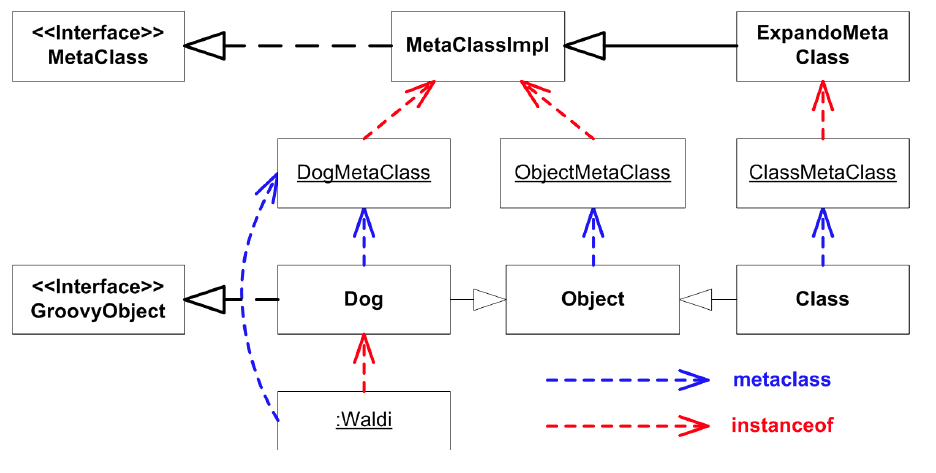
\includegraphics[width=0.8\textwidth]{pics/groovyMetaklassen}
	\end{center}
	\caption{Beziehung von Metaklassen, Klassen und Instanzen \cite{mpInGroovy})}
	\label{groovyMetaclassDiagram}
\end{figure}




\subsection{Closures} 


\subsection{Kategorien}
Mit Kategorien bietet Groovy eine Art dynamische Mix-ins. Es können innerhalb
von einem Closure, beliebige Methoden zu allen Metaklassen hinzugefügt oder
überschrieben werden.
Die Methode use ist eine der Standardmethoden in DefaultGroovyMethods die jeder
Metaklasse, die von MetaClassImpl erbt, automatisch hinzugefügt wird. Deswegen
wird häufig von use auch von einem Sprachkonstrukt statt von einer Methode
gesprochen. Mit use wird die in Klammern angegebene Klasse auf Klas- senmethoden
untersucht und in org.codehaus.groovy.runtime.GroovyCategory- Support verwaltet.
Es werden nur Klassenmethoden erlaubt, um Zustände in der Kategoriein- stanz zu
vermeiden, die nicht threadsicher wären. Der this Parameter wird des- halb bei
Üerschreiben von Instanzmethoden wie getName explizit als ersten Parameter
angegeben. Wird nun eine Methode aufgerufen, überprüft MetaClas- sImpl in
invokeMethod ob es eine Kategorie Methode gibt, die kompatibel ist mit dem
aktuellen Objekt und den übergebenen Parametern. Gibt es solch eine wird der
Aufruf delegiert, sonst wird wie in 2.5 beschrieben der normale Aufruf
fortgesetzt.
Kategorien sind von Objective-C entlehnt und bieten eine einfache Mög-
lichkeit, kurzzeitig und ohne Seiteneffekte neue Methoden hinzuzufügen oder
bestehende zu überschreiben. Sie eignen sich deswegen gut für Aspekt- oder
Contextorientierte Programmierung. \cite{mpInGroovy}
\subsection{Expando-MetaClass}


\chapter{MDA / MDSD und DSM Unterschiede} 
%begin copy
Model-driven Architecture (MDA) bzw. Model-Driven Software Development (MDSD)
und Me- taprogrammierung bzw. DSLs haben eine vergleichbare Problemstellung. In
der MDA Welt ver- wendet man auf UML etc. basierende graphische Modele. Auch das
graphische Model muss eine formale Sprache sein, damit es compilerbar ist. Eine
DSL kann man als textuelle Repräsentation eines Models verstehen.
Die Komplexität und das Abstraktionsniveau ist abhängig von dem verwendeten
Model, nicht seiner Repräsentation. Graphische Repräsentation kann man aber
besser mit zusätzlichen Infor- mationen anreichern, da man diese nach Bedarf
ein- und ausblenden kann.
Eine DSL hat den Vorteil, das ihre Darstellung simpler ist, man kann sie
beispielsweise mit einem einfachen Text Editor bearbeiten oder mit trivialen
Mitteln ein diff zweier Versionen erstellen (vgl. Sachez Cuadrado and
Jesu \ldots. Building domain-specific languages for model-driven
development. IEEE Softw., 24(5):48–55, 2007. \& Diomidis Spinellis. Rational
metaprogramming. IEEE Software, 25(1):78–79, January/Fe- bruary 2008.).
 (vgl. \cite{biekermetaprogrammierung})
 %end copy
 
 
 %begin copy -- wie funktioniert eine dsl
 In unserem Beispiel mit der Uhrenanwendung sind die
Domänenkonzepte hergeleitet aus der visuellen Anzeige (z.
B. Zeiteinheiten, Symbole etc.), der Kontrollstruktur (Nutzer
drückt Knopf, Alarm wird ausgelöst etc.) und darunter liegenden
Diensten (d. h. Zeit und ihre Manipulation, Alarm). Indem
diese Konzepte in die Modellierungssprache eingebracht und
weiter verfeinert werden, erzeugen wir die Spezifikation der
Sprache (d. h. das Metamodell). Das Ziel ist hier, die gewählten
Konzepte akkurat auf die Semantik der Domäne abzubilden. \cite{dsmUhrenArtikel}
 %end copy
 
 
  
 %begin copy -- unterschiede dsm und mda
Wie unterscheidet sich DSM von MDA?
Nachdem wir mit Beispielen die Hauptprinzipien von domänenspezifischer
Modellierung demonstriert haben, können wir
sie nun mit anderen gängigen modellbasierten Entwicklungsansätzen
vergleichen und speziell mit der Model Driven Architecture
(MDA) der OMG. Ganz grundsätzlich beinhaltet MDA
die Umwandlung von UML-Modellen auf einem höheren Abstraktionsniveau
in UML-Modelle auf einem niedrigeren Abstraktionsniveau.
Gewöhnlich sind dies zwei Ebenen, und zwar
plattformunabhängige Modelle (PIMs) und plattformspezifische
Modelle (PSMs). Diese PIMs und PSMs sind reines UML
und bieten daher keine wirkliche Erhöhung der Abstraktion.
In der MDA werden auf jeder Stufe die Modelle einer detaillierteren
Bearbeitung mit Reverse und Roundtrip Engineering
unterzogen und am Ende wird wesentlicher Code aus dem finalen
Modell generiert. Die OMG verfolgt mit MDA das Ziel,
dasselbe PIM auf verschiedenen Software-Plattformen nutzen
zu können. Außerdem will die OMG alle Übersetzungen und
Modellformate standardisieren, sodass die Modelle zwischen
den Werkzeugen verschiedener Hersteller austauschbar werden.
Dies erreichen zu wollen, ist sehr ambitioniert, aber man
ist noch viele Jahre davon entfernt. Diese Zielsetzung zeigt jedoch
klar die Unterschiede zwischen DSM und MDA und beantwortet
die Frage, wann welcher Ansatz anzuwenden ist.
DSM erfordert Domänen-Fachwissen, ein Potenzial, das eine
Firma nur erreichen kann, wenn sie kontinuierlich in der gleichen
Problemdomäne arbeitet. Dies sind typischerweise eher
Produkt- oder Systementwicklungshäuser als Projekthäuser.
Hier ist die Plattformunabhängigkeit keine wichtige Anforderung, obwohl sie mit DSM einfach erreicht werden kann, indem
verschiedene Code-Generatoren für verschiedene Softwareund/
oder Produktplattformen eingesetzt werden. Stattdessen
liegt das Hauptaugenmerk der DSM auf der signifikanten Verbesserung
der Entwicklerproduktivität.
Mit der MDA richtet die OMG ihren Fokus nicht auf die Nutzung
von DSM-Sprachen, sondern auf generisches UML, ihre
eigene Standard-Modellierungssprache. Sie versucht nicht, das
möglicherweise existierende Domänen-Fachwissen einer Firma
einzukapseln, sondern nimmt an, dass dieses Wissen nicht
vorhanden oder irrelevant ist. Es scheint daher, dass die MDA,
wenn die OMG letztlich ihre selbstgesteckten Ziele erreicht, geeignet
für System- oder Anwendungsintegrationsprojekte ist.
MDA setzt ein fundiertes Wissen ihrer Methodik voraus,
welches nicht per se in einer Firma vorhanden ist und durch
Erfahrung erlangt werden muss. Folglich muss das MDAFachwissen
angeeignet oder von außerhalb eingekauft werden,
wohingegen das Domänen-Fachwissen für die DSM schon in
einer Organisation verfügbar ist und angewendet wird. In diesen
Situationen ist die Wahl zwischen MDA und DSM oft klar.
 \cite{dsmUhrenArtikel}
 %end copy
 
 
 
\chapter{Praktischer Teil}
Der praktische Teil beschäftigt sich nun mit \ldots

\section{Die Fachliche Domäne}

\chapter{Auswertung}

\chapter{Zusammenfassung und Schlussbetrachtung}

 %begin copy -- unterschiede dsm und mda
Domänenspezifische Modellierung erlaubt schnellere Entwicklung
basierend auf den Modellen der Problemdomäne und weniger auf
Modellen von Quellcode. Unser Uhrenbeispiel veranschaulichte dies
schnell. Industrielle Erfahrungen mit DSM [DSM] zeigen bedeutende
Verbesserungen der Produktivität, niedrigere Entwicklungskosten
und bessere Qualität. Das Unternehmen Nokia gibt beispielsweise
an, dass sich die Entwicklung von Mobiltelefonen auf
diesem Weg um den Faktor 10 beschleunigt. Bei der Firma Lucent
konnte die Produktivität – abhängig vom Produkt – um das drei- bis
zehnfache gesteigert werden. Die Schlüsselfaktoren dafür sind:
H Das Problem wird nur einmal – und zwar auf einem hohen
Abstraktionsniveau – gelöst und der lauffähige Quellcode
wird geradewegs aus dieser Lösung generiert.
H Das Hauptaugenmerk der Entwickler liegt nicht länger auf dem
Code, sondern beim Modell, dem Problem an sich. Komplexität
und Implementierungsdetails können so verborgen werden und
eine bereits bekannte Terminologie rückt in den Vordergrund.
H Durch eine einheitlichere Entwicklungsumgebung und dadurch,
dass weniger Wechsel zwischen den Abstraktionsniveaus
Modell und Implementierung erforderlich sind, lassen
sich eine bessere Konsistenz der verschiedenen Produkte
und niedrigere Fehlerraten erreichen.
H Das Domänenwissen wird für das Entwicklungsteam explizit
gemacht, indem es in der Modellierungssprache und deren
Werkzeugunterstützung festgehalten wird.
Der Einsatz von DSM bedeutet keine zusätzliche Investition,
wenn der gesamte Zyklus vom Design bis zum arbeitenden
Code betrachtet wird. Vielmehr spart es Entwicklungsressourcen:
Traditionell arbeiten alle Entwickler mit den Konzepten der
Problemdomäne und bilden diese von Hand auf die Implementierungskonzepte
ab. Aber unter den Entwicklern gibt es große
Unterschiede. Manche erledigen diese Aufgabe besser, manche
schlechter. Also lasst die erfahrenen Entwickler die Konzepte
und deren Abbildung einmal definieren, dann müssen die anderen
dies nicht erneut tun. Spezifiziert ein Experte den Code-
Generator, so produziert dieser Anwendungen von besserer
Qualität, als es normale Entwickler von Hand könnten.
 \cite{dsmUhrenArtikel}
 %end copy
 
 
\bibliographystyle{alphadin}
\clearpage\addcontentsline{toc}{chapter}{\bibname}\bibliography{jabref}
\appendix
\renewcommand{\theequation}{A-\arabic{equation}}

\setcounter{equation}{0}  % reset counter \chapter*{Anhang}  % use *-form to

%\chapter{Anhang}
\addcontentsline{toc}{chapter}{Anhang}

%\section{Anhang A - Screenshots}\label{appendixA}


%\listoffigures
\end{document}
